% \newpage

\section{Alternative case study: concrete beam}

The alternative case study still considers a beam supporting a hollow-core slab floor in an an office building.
However, this is now a reinforced concrete beam, with the effective beam depth as the decision parameter $x$, see Figure \ref{fig:beam_concrete} below.
This problem was adapted from \citep{Hingorani2025Resource-EfficientConcepts}, with data on material cost and emissions gathered from \citep{UniconPRICE2024}.

\begin{figure}[h]
    \centering
    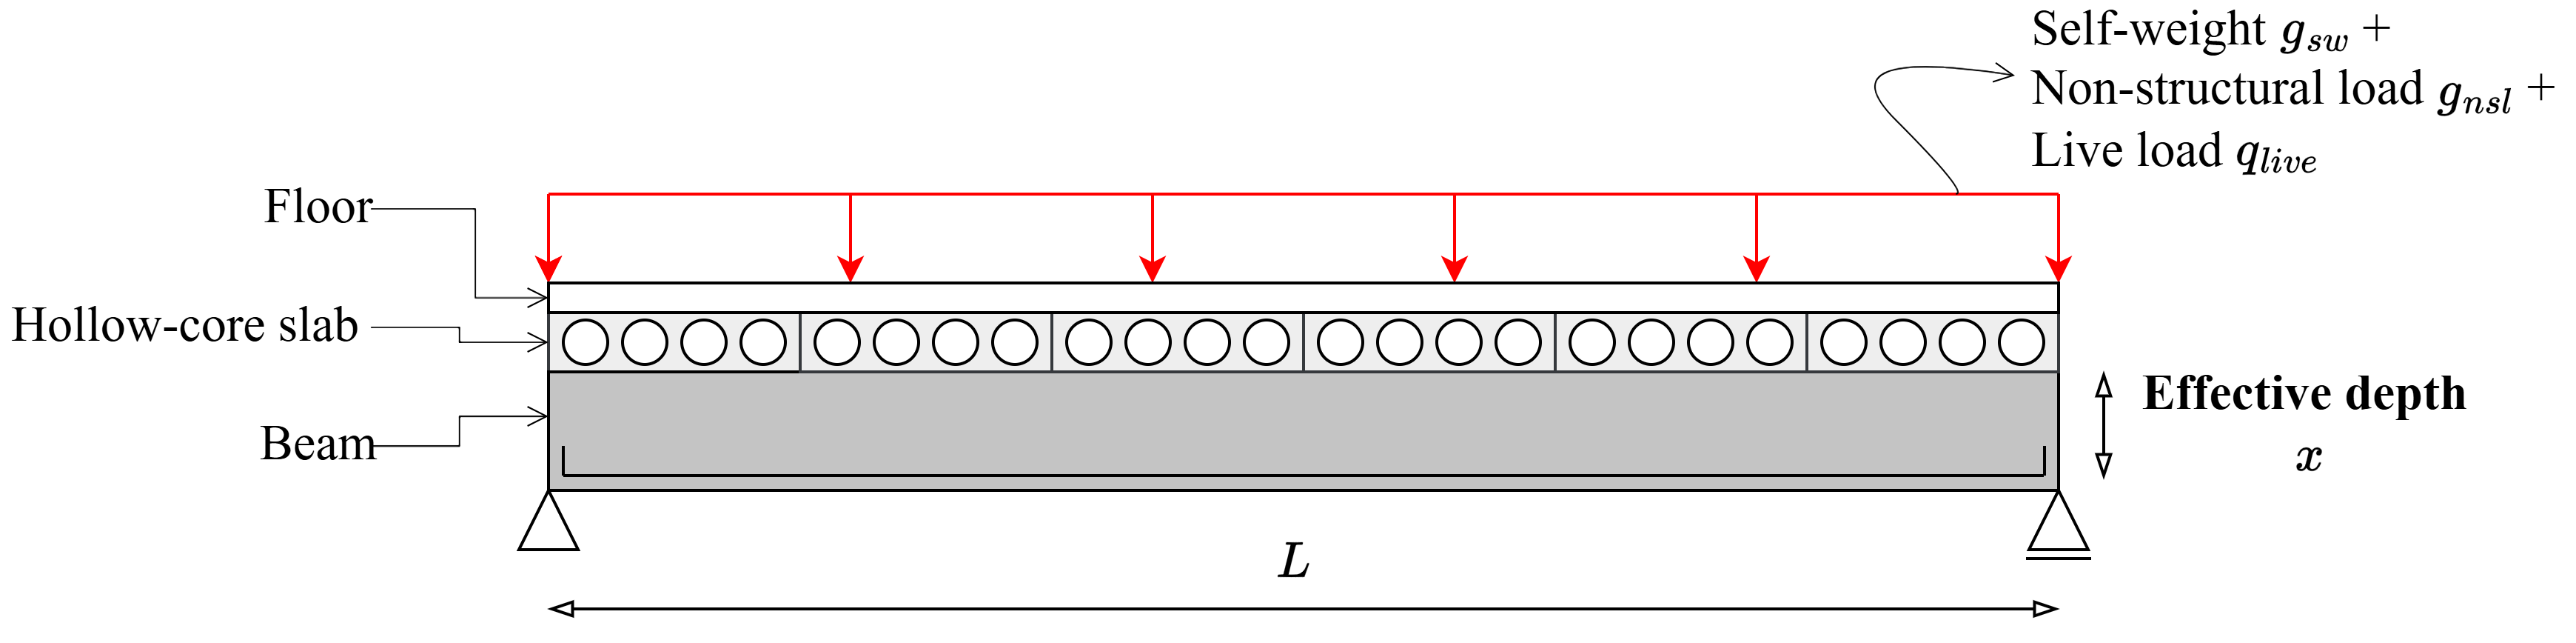
\includegraphics[width=0.8\linewidth]{Images/beam_concrete_variant.png}
    \caption{The alternative case study, with the loads, dimensions and decision variable indicated. Not to scale.}
    \label{fig:beam_concrete}
\end{figure}

The limit state function for the bending failure mechanism of this structure is:

\begin{equation}
    \label{eqn:LSF_alt}
    Z = \theta_R b \rho_s x^2 f_y \left( 1 - \frac{1}{2} \rho_s \frac{f_y}{f_c} \right) - \theta_E \frac{(g_{sw} + g_{nsl} + \theta_q q_{live})DL^2}{8}
\end{equation}

With $b$ the beam width and $\rho_s$ the reinforcement ratio, both deterministic, while the reinforcement yield strength $f_y$ and concrete compressive strength $f_c$ (class C30/37) are stochastic variables.
The other parameters are identical to Equation \ref{eqn:LSF}, though the distribution of the resistance model uncertainty $\theta_R$ has been adjusted to the specific resistance model.
The full probabilistic model of this structure is described in Table \ref{tab:distributions_concrete}.
The parameter values of the cost and emission functions are given in Table \ref{tab:C_E_params_concrete}.
The `push'-parameters $C_1$ and $E_1$ are again based on a linear relation between the decision variable and beam volume, with a material cost of $\EUR{}$ 0.10/kg concrete, and emission intensity of 0.11 kg CO\textsubscript{2}eq/kg concrete.
Note that the parameter $E_1$ is adjusted to adhere to the emission-cost ratio for which this alternative case study is considered.
The $x$-independent variables $C_0$ and $E_0$ are based on the same assumptions as for the original steel variant of the case study, with a small increase to account for the concrete volume below the effective depth of the beam (based on an assumed concrete cover of 30 mm, independent of $x$).
Finally, the 'pull' parameters $C_H$ and $E_H$ are identical to the original steel variant of the case study.

\begin{table}[h]
    \centering
    
    \begin{tabular}{c|c|c|c|c|c}
         Variable & Description & Unit & Distribution & Mean & CoV  \\ \hline
         $q_{live}$& Variable load & kN/m\textsuperscript{2}& Gumbel & 1.2&0.5\\
         $g_{sw}$& Self-weight load& kN/m\textsuperscript{2}& Normal& 4.137& 0.1\\
         $g_{nsl}$& Non-structural load& kN/m\textsuperscript{2}& Normal& 2.8&0.1\\
         $f_y$& Yield strength reinforcement steel& N/mm\textsuperscript{2}& Lognormal& 538.4&0.045\\
 $f_c$& Concrete compressive strength& N/mm\textsuperscript{2}& Lognormal& 35.4&0.1\\
         $\theta_R$& Resistance model uncertainty&-& Lognormal& 1.035&0.07\\
         $\theta_E$& Load effect model uncertainty&-& Lognormal& 1.0&0.1\\
         $\theta_q$& Live load model uncertainty&-& Lognormal& 1.0&0.1\\
         $L$ & Beam length & m & Deterministic & 12 & - \\
         $D$ & Beam spacing & m & Deterministic & 12 & - \\
 $b$& Beam width& mm& Deterministic & 500&-\\
 $\rho_s$& Reinforcement ratio& -& Deterministic & 0.05&-\\
         $x$& Effective beam depth& mm& Deterministic & \emph{To be optimised} & - \\
    \end{tabular}
 \caption{Distributions of random variables in the limit state function used in the concrete variant of the case study, derived from \citep{Vrouwenvelder2024ReliabilityEurocodes,Hingorani2023TowardsDesign}.}   \label{tab:distributions_concrete}
\end{table}

\begin{table}[h]
    \centering
    \begin{tabular}{c|c|c|c}
         Parameter & Description& unit  &value 
\\ \hline
 $C_0$& $x$-independent costs& EUR  &1.05*10\textsuperscript{3}\\
 $C_1$& $x$-dependent costs&EUR$/mm^3$ &1.60*10\textsuperscript{-5}\\
 $C_H$& Additional failure costs&EUR &2.70*10\textsuperscript{6}
\\
 $E_0$& $x$-independent emissions&kg CO\textsubscript{2}eq &3.84*10\textsuperscript{2}\\
 $E_1$& $x$-dependent emissions&kg CO\textsubscript{2}eq/$mm^3$ &1.78*10\textsuperscript{-5}\\
 $E_H$& Additional failure emissions&kg CO\textsubscript{2}eq &6.65*10\textsuperscript{4}\\\end{tabular}
    \caption{Parameter values in the cost and emission functions for the concrete variant of the case study}
    \label{tab:C_E_params_concrete}
\end{table}

